\documentclass[usenames,dvipsnames,aspectratio=169]{beamer}
\usepackage{../common/prg}

\title[11. előadás]{Programozás}
\subtitle{(GKxB\_INTM114)}

\begin{document}

%1
\begin{frame}[plain]
  \titlepage
  \logoalul
\end{frame}

%2
\section{Egyszeresen láncolt lista}
\subsection{Verem megvalósítása listával}
\begin{frame}
  Verem megvalósítható tömbbel, de annak mérete véges, fordítási időben adott.
  Lehetséges megoldás: \hiv{\href{https://hu.wikipedia.org/wiki/L\%C3\%A1ncolt_lista}{láncolt lista}} (Linked List, önhivatkozó adatszerkezet)
  \begin{center}
    
\includegraphics[scale=0.8]{list1.pdf}\\
    \scriptsize
    Egyszeresen láncolt lista (Singly Linked List)
  \end{center}
  \begin{exampleblock}{Felhasználható struktúra}
    \footnotesize
    struct Lista1 \{\\
    \qquad \kiemel{ADAT} adat;\\
    \qquad Lista1 *kov;\\
    \};\\
  \end{exampleblock}
\end{frame}

%3
\begin{frame}
  \scriptsize
  \begin{columns}[T]
    \column{0.7\textwidth}
      \begin{exampleblock}{\textattachfile{veremTeszt2.cpp}{veremTeszt2.cpp}}
        \scriptsize
        \vspace{-0.3cm}
        \lstinputlisting[style=cpp,numbers=left]{veremTeszt2.cpp}
        \vspace{-0.3cm}
      \end{exampleblock}
    \column{0.25\textwidth}
      \begin{exampleblock}{\textattachfile{verem2.h}{verem2.h}}
        \normalsize
        \lstinputlisting[style=cpp,linerange={4-7},numbers=right,firstnumber=4]{verem2.h}
      \end{exampleblock}
  \end{columns}
\end{frame}

%%%%%%%%%%%%%%%%%%%%%%%%%%%%%%%%%%%
%%%%%%%%%%%%%%%%%%%%%%%%%%%%%%%%%%%

%4
\subsection{Új elemek verembe helyezése (push)}
\begin{frame}
  \begin{columns}[c]
    \column{0.5\textwidth}
      \begin{exampleblock}{\textattachfile{verem2.cpp}{verem2.cpp}}
        \vspace{-.2cm}
        \small
        \lstinputlisting[style=cpp,linerange={4-16},numbers=left,firstnumber=4]{verem2.cpp}
        \vspace{-.2cm}
      \end{exampleblock}
    \column{0.45\textwidth}
      
\includegraphics[width=\textwidth]{verem/verem01.pdf}
  \end{columns}
\end{frame}

%5
\begin{frame}
  \begin{columns}[c]
    \column{0.5\textwidth}
      \begin{exampleblock}{\textattachfile{verem2.cpp}{verem2.cpp}}
        \vspace{-.2cm}
        \small
        \lstinputlisting[style=cpp,linerange={4-16},numbers=left,firstnumber=4]{verem2.cpp}
        \vspace{-.2cm}
      \end{exampleblock}
    \column{0.45\textwidth}
      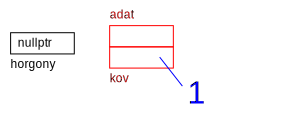
\includegraphics[width=\textwidth]{verem/verem02.pdf}
  \end{columns}
\end{frame}

%6
\begin{frame}
  \begin{columns}[c]
    \column{0.5\textwidth}
      \begin{exampleblock}{\textattachfile{verem2.cpp}{verem2.cpp}}
        \vspace{-.2cm}
        \small
        \lstinputlisting[style=cpp,linerange={4-16},numbers=left,firstnumber=4]{verem2.cpp}
        \vspace{-.2cm}
      \end{exampleblock}
    \column{0.45\textwidth}
      \includegraphics[width=\textwidth]{verem/verem03.pdf}
  \end{columns}
\end{frame}

%7
\begin{frame}
  \begin{columns}[c]
    \column{0.5\textwidth}
      \begin{exampleblock}{\textattachfile{verem2.cpp}{verem2.cpp}}
        \vspace{-.2cm}
        \small
        \lstinputlisting[style=cpp,linerange={4-16},numbers=left,firstnumber=4]{verem2.cpp}
        \vspace{-.2cm}
      \end{exampleblock}
    \column{0.45\textwidth}
      \includegraphics[width=\textwidth]{verem/verem04.pdf}
  \end{columns}
\end{frame}

%8
\begin{frame}
  \begin{columns}[c]
    \column{0.5\textwidth}
      \begin{exampleblock}{\textattachfile{verem2.cpp}{verem2.cpp}}
        \vspace{-.2cm}
        \small
        \lstinputlisting[style=cpp,linerange={4-16},numbers=left,firstnumber=4]{verem2.cpp}
        \vspace{-.2cm}
      \end{exampleblock}
    \column{0.45\textwidth}
      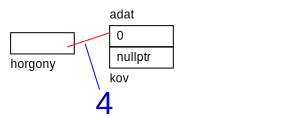
\includegraphics[width=\textwidth]{verem/verem05.pdf}
  \end{columns}
\end{frame}

%9
\begin{frame}
  \begin{columns}[c]
    \column{0.5\textwidth}
      \begin{exampleblock}{\textattachfile{verem2.cpp}{verem2.cpp}}
        \vspace{-.2cm}
        \small
        \lstinputlisting[style=cpp,linerange={4-16},numbers=left,firstnumber=4]{verem2.cpp}
        \vspace{-.2cm}
      \end{exampleblock}
    \column{0.45\textwidth}
      \includegraphics[width=\textwidth]{verem/verem06.pdf}
  \end{columns}
\end{frame}

%10
\begin{frame}
  \begin{columns}[c]
    \column{0.5\textwidth}
      \begin{exampleblock}{\textattachfile{verem2.cpp}{verem2.cpp}}
        \vspace{-.2cm}
        \small
        \lstinputlisting[style=cpp,linerange={4-16},numbers=left,firstnumber=4]{verem2.cpp}
        \vspace{-.2cm}
      \end{exampleblock}
    \column{0.45\textwidth}
      \includegraphics[width=\textwidth]{verem/verem07.pdf}
  \end{columns}
\end{frame}

%11
\begin{frame}
  \begin{columns}[c]
    \column{0.5\textwidth}
      \begin{exampleblock}{\textattachfile{verem2.cpp}{verem2.cpp}}
        \vspace{-.2cm}
        \small
        \lstinputlisting[style=cpp,linerange={4-16},numbers=left,firstnumber=4]{verem2.cpp}
        \vspace{-.2cm}
      \end{exampleblock}
    \column{0.45\textwidth}
      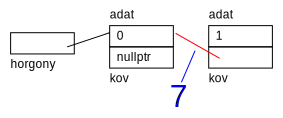
\includegraphics[width=\textwidth]{verem/verem08.pdf}
  \end{columns}
\end{frame}

%12
\begin{frame}
  \begin{columns}[c]
    \column{0.5\textwidth}
      \begin{exampleblock}{\textattachfile{verem2.cpp}{verem2.cpp}}
        \vspace{-.2cm}
        \small
        \lstinputlisting[style=cpp,linerange={4-16},numbers=left,firstnumber=4]{verem2.cpp}
        \vspace{-.2cm}
      \end{exampleblock}
    \column{0.45\textwidth}
      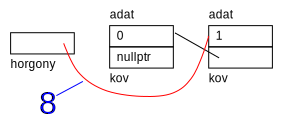
\includegraphics[width=\textwidth]{verem/verem09.pdf}
  \end{columns}
\end{frame}


%%%%%%%%%%%%%%%%%%%%%%%%%%%%%%%%%%%
%%%%%%%%%%%%%%%%%%%%%%%%%%%%%%%%%%%

%13
\subsection{Elemek eltávolítása a veremből (pop)}
\begin{frame}
  \begin{columns}[c]
    \column{0.5\textwidth}
      \footnotesize
      \begin{exampleblock}{\textattachfile{verem2.cpp}{verem2.cpp}}
        \lstinputlisting[style=cpp,linerange={18-29},numbers=left,firstnumber=19]{verem2.cpp}
      \end{exampleblock}
    \column{0.45\textwidth}
      \includegraphics[width=\textwidth]{verem/verem10.pdf}
  \end{columns}
\end{frame}

%14
\begin{frame}
  \begin{columns}[c]
    \column{0.5\textwidth}
      \footnotesize
      \begin{exampleblock}{\textattachfile{verem2.cpp}{verem2.cpp}}
        \lstinputlisting[style=cpp,linerange={18-29},numbers=left,firstnumber=19]{verem2.cpp}
      \end{exampleblock}
    \column{0.45\textwidth}
      \includegraphics[width=\textwidth]{verem/verem11.pdf}
  \end{columns}
\end{frame}

%15
\begin{frame}
  \begin{columns}[c]
    \column{0.5\textwidth}
      \footnotesize
      \begin{exampleblock}{\textattachfile{verem2.cpp}{verem2.cpp}}
        \lstinputlisting[style=cpp,linerange={18-29},numbers=left,firstnumber=19]{verem2.cpp}
      \end{exampleblock}
    \column{0.45\textwidth}
      \includegraphics[width=\textwidth]{verem/verem12.pdf}
  \end{columns}
\end{frame}

%16
\begin{frame}
  \begin{columns}[c]
    \column{0.5\textwidth}
      \footnotesize
      \begin{exampleblock}{\textattachfile{verem2.cpp}{verem2.cpp}}
        \lstinputlisting[style=cpp,linerange={18-29},numbers=left,firstnumber=19]{verem2.cpp}
      \end{exampleblock}
    \column{0.45\textwidth}
      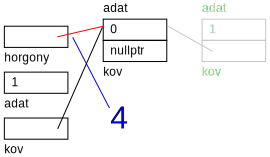
\includegraphics[width=\textwidth]{verem/verem13.pdf}
  \end{columns}
\end{frame}

%17
\begin{frame}
  \begin{columns}[c]
    \column{0.5\textwidth}
      \footnotesize
      \begin{exampleblock}{\textattachfile{verem2.cpp}{verem2.cpp}}
        \lstinputlisting[style=cpp,linerange={18-29},numbers=left,firstnumber=19]{verem2.cpp}
      \end{exampleblock}
    \column{0.45\textwidth}
      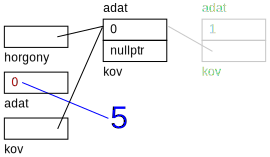
\includegraphics[width=\textwidth]{verem/verem14.pdf}
  \end{columns}
\end{frame}

%18
\begin{frame}
  \begin{columns}[c]
    \column{0.5\textwidth}
      \footnotesize
      \begin{exampleblock}{\textattachfile{verem2.cpp}{verem2.cpp}}
        \lstinputlisting[style=cpp,linerange={18-29},numbers=left,firstnumber=19]{verem2.cpp}
      \end{exampleblock}
    \column{0.45\textwidth}
      \includegraphics[width=\textwidth]{verem/verem15.pdf}
  \end{columns}
\end{frame}

%19
\begin{frame}
  \begin{columns}[c]
    \column{0.5\textwidth}
      \footnotesize
      \begin{exampleblock}{\textattachfile{verem2.cpp}{verem2.cpp}}
        \lstinputlisting[style=cpp,linerange={18-29},numbers=left,firstnumber=19]{verem2.cpp}
      \end{exampleblock}
    \column{0.45\textwidth}
      \includegraphics[width=\textwidth]{verem/verem16.pdf}
  \end{columns}
\end{frame}

%20
\begin{frame}
  \begin{columns}[c]
    \column{0.5\textwidth}
      \footnotesize
      \begin{exampleblock}{\textattachfile{verem2.cpp}{verem2.cpp}}
        \lstinputlisting[style=cpp,linerange={18-29},numbers=left,firstnumber=19]{verem2.cpp}
      \end{exampleblock}
    \column{0.45\textwidth}
      \includegraphics[width=\textwidth]{verem/verem17.pdf}
  \end{columns}
\end{frame}

%%%%%%%%%%%%%%%%%%%%%%%%%%%%%%%%%%%
%%%%%%%%%%%%%%%%%%%%%%%%%%%%%%%%%%%

%21
\subsection{Néhány általános listaművelet megvalósítása}
\begin{frame}
  Készítsünk általánosan használható függvényeket egyszeresen láncolt lista manipulálásához!
  \scriptsize
  \begin{exampleblock}{\textattachfile{listaTeszt1.cpp}{listaTeszt1.cpp} (\textattachfile{Lista1.cpp}{Lista1.cpp}, %
  \textattachfile{Lista1.h}{Lista1.h})}
    \meret{7}
    \vspace{-0.2cm}
    \lstinputlisting[style=cpp,numbers=left]{listaTeszt1.cpp}
    \vspace{-0.2cm}
  \end{exampleblock}
\end{frame}

%%%%%%%%%%%%%%%%%%%%%%%%%%%%%%%%%%%
%%%%%%%%%%%%%%%%%%%%%%%%%%%%%%%%%%%

%22
\subsection{Új elem beillesztése adott elem után}
\begin{frame}
  \begin{center}
    \includegraphics[scale=0.6]{lista1/list1-01.pdf}
  \end{center}
  \vspace{-.2cm}
  \meret{7}
  \begin{exampleblock}{\textattachfile{Lista1.cpp}{Lista1.cpp}}
    \vspace{-.2cm}
    \lstinputlisting[style=cpp,linerange={5-18},numbers=left,firstnumber=5]{Lista1.cpp}
    \vspace{-.2cm}
  \end{exampleblock}
\end{frame}

%23
\begin{frame}
  \begin{center}
    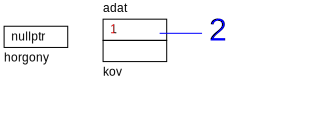
\includegraphics[scale=0.6]{lista1/list1-02.pdf}
  \end{center}
  \vspace{-.2cm}
  \meret{7}
  \begin{exampleblock}{\textattachfile{Lista1.cpp}{Lista1.cpp}}
    \vspace{-.2cm}
    \lstinputlisting[style=cpp,linerange={5-18},numbers=left,firstnumber=5]{Lista1.cpp}
    \vspace{-.2cm}
  \end{exampleblock}
\end{frame}

%24
\begin{frame}
  \begin{center}
    \includegraphics[scale=0.6]{lista1/list1-03.pdf}
  \end{center}
  \vspace{-.2cm}
  \meret{7}
  \begin{exampleblock}{\textattachfile{Lista1.cpp}{Lista1.cpp}}
    \vspace{-.2cm}
    \lstinputlisting[style=cpp,linerange={5-18},numbers=left,firstnumber=5]{Lista1.cpp}
    \vspace{-.2cm}
  \end{exampleblock}
\end{frame}

%25
\begin{frame}
  \begin{center}
    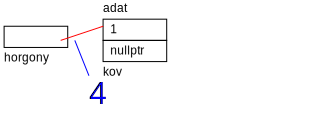
\includegraphics[scale=0.6]{lista1/list1-04.pdf}
  \end{center}
  \vspace{-.2cm}
  \meret{7}
  \begin{exampleblock}{\textattachfile{listaTeszt1.cpp}{listaTeszt1.cpp}}
    \vspace{-.2cm}
    \lstinputlisting[style=cpp,linerange={6-18},numbers=left,firstnumber=6]{listaTeszt1.cpp}
    \vspace{-.2cm}
  \end{exampleblock}
\end{frame}

%26
\begin{frame}
  \begin{center}
    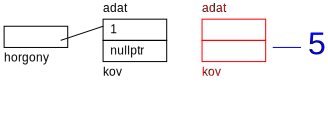
\includegraphics[scale=0.6]{lista1/list1-05.pdf}
  \end{center}
  \vspace{-.2cm}
  \meret{7}
  \begin{exampleblock}{\textattachfile{Lista1.cpp}{Lista1.cpp}}
    \vspace{-.2cm}
    \lstinputlisting[style=cpp,linerange={5-18},numbers=left,firstnumber=5]{Lista1.cpp}
    \vspace{-.2cm}
  \end{exampleblock}
\end{frame}

%27
\begin{frame}
  \begin{center}
    \includegraphics[scale=0.6]{lista1/list1-06.pdf}
  \end{center}
  \vspace{-.2cm}
  \meret{7}
  \begin{exampleblock}{\textattachfile{Lista1.cpp}{Lista1.cpp}}
    \vspace{-.2cm}
    \lstinputlisting[style=cpp,linerange={5-18},numbers=left,firstnumber=5]{Lista1.cpp}
    \vspace{-.2cm}
  \end{exampleblock}
\end{frame}

%28
\begin{frame}
  \begin{center}
    \includegraphics[scale=0.6]{lista1/list1-07.pdf}
  \end{center}
  \vspace{-.2cm}
  \meret{7}
  \begin{exampleblock}{\textattachfile{Lista1.cpp}{Lista1.cpp}}
    \vspace{-.2cm}
    \lstinputlisting[style=cpp,linerange={5-18},numbers=left,firstnumber=5]{Lista1.cpp}
    \vspace{-.2cm}
  \end{exampleblock}
\end{frame}

%29
\begin{frame}
  \begin{center}
    \includegraphics[scale=0.6]{lista1/list1-08.pdf}
  \end{center}
  \vspace{-.2cm}
  \meret{7}
  \begin{exampleblock}{\textattachfile{listaTeszt1.cpp}{listaTeszt1.cpp}}
    \vspace{-.2cm}
    \lstinputlisting[style=cpp,linerange={6-18},numbers=left,firstnumber=6]{listaTeszt1.cpp}
    \vspace{-.2cm}
  \end{exampleblock}
\end{frame}

%%%%%%%%%%%%%%%%%%%%%%%%%%%%%%%%%%%
%%%%%%%%%%%%%%%%%%%%%%%%%%%%%%%%%%%

%30
\subsection{Egyszeresen láncolt lista bejárása}
\begin{frame}[fragile]
  \scriptsize
  \begin{columns}[t]
    \column{.49\textwidth}
      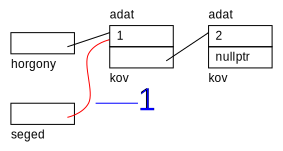
\includegraphics[scale=.7]{lista1/list1-10.pdf} \\
      \vspace{1cm}
      \includegraphics[scale=.7]{lista1/list1-12.pdf}
    \column{.49\textwidth}
      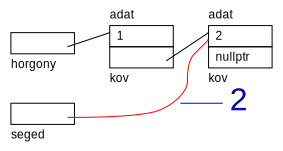
\includegraphics[scale=.7]{lista1/list1-11.pdf} \\
      \begin{exampleblock}{\textattachfile{Lista1.cpp}{Lista1.cpp}}
        \scriptsize
        \lstinputlisting[style=cpp,linerange={20-27},numbers=right,firstnumber=20]{Lista1.cpp}
      \end{exampleblock}
  \end{columns}
\end{frame}

%31
\subsection{Egyszeresen láncolt lista törlése}
\begin{frame}[fragile]
  \scriptsize
  \begin{columns}[T]
    \column{.4\textwidth}
      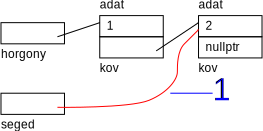
\includegraphics[scale=.6]{lista1/list1-20.pdf} \\
      \hrulefill \\
      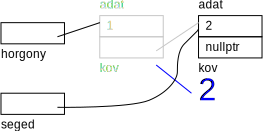
\includegraphics[scale=.6]{lista1/list1-21.pdf} \\
      \hrulefill \\
      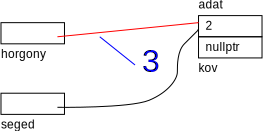
\includegraphics[scale=.6]{lista1/list1-22.pdf}
    \column{.55\textwidth}
      \begin{exampleblock}{\textattachfile{Lista1.cpp}{Lista1.cpp}}
        \small
        \lstinputlisting[style=cpp,linerange={31-38},numbers=right,firstnumber=38]{Lista1.cpp}
      \end{exampleblock}
  \end{columns}
\end{frame}

%32
\begin{frame}[fragile]
  \scriptsize
  \begin{columns}[T]
    \column{.4\textwidth}
      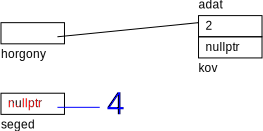
\includegraphics[scale=.6]{lista1/list1-23.pdf} \\
      \hrulefill \\
      \includegraphics[scale=.6]{lista1/list1-24.pdf} \\
      \hrulefill \\
      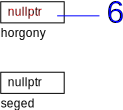
\includegraphics[scale=.6]{lista1/list1-25.pdf}
    \column{.55\textwidth}
      \begin{exampleblock}{\textattachfile{Lista1.cpp}{Lista1.cpp}}
        \small
        \lstinputlisting[style=cpp,linerange={31-38},numbers=right,firstnumber=38]{Lista1.cpp}
      \end{exampleblock}
  \end{columns}
\end{frame}

%33
\section{Kétszeresen láncolt lista}
\subsection{Sor megvalósítása listával}
\begin{frame}
  \small
  Készítsük el a verem mintájára a sor megvalósítását is láncolt listával!\\
  Probléma: a lista utolsó elemének eltávolítása nehézkes.\\
  Megoldás: kétszeresen láncolt lista.
  \begin{center}
    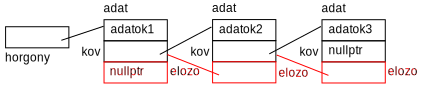
\includegraphics[scale=0.8]{list2.pdf} \\
    \tiny
    Kétszeresen láncolt lista (Doubly Linked List)
  \end{center}
  \begin{exampleblock}{Felhasználható struktúra}
    \scriptsize
    struct Lista2 \{\\    
    \qquad \kiemel{ADAT} adat;\\
    \qquad Lista2 *elozo, *kov;\\
    \};\\
  \end{exampleblock}
\end{frame}

%34
\begin{frame}
  \scriptsize
  \begin{columns}[T]
    \column{0.6\textwidth}
      \begin{exampleblock}{\textattachfile{sorTeszt2.cpp}{sorTeszt2.cpp}}
        \scriptsize
        \vspace{-0.2cm}
        \lstinputlisting[style=cpp,numbers=left]{sorTeszt2.cpp}
        \vspace{-0.2cm}
      \end{exampleblock}
    \column{0.35\textwidth}
      \begin{exampleblock}{\textattachfile{sor2.h}{sor2.h}}
        \small
        \lstinputlisting[style=cpp,linerange={4-7},numbers=right,firstnumber=4]{sor2.h}
      \end{exampleblock}
  \end{columns}
\end{frame}

%%%%%%%%%%%%%%%%%%%%%%%%%%%%%%%%%%%
%%%%%%%%%%%%%%%%%%%%%%%%%%%%%%%%%%%

%35
\subsection{Új elemek sorba helyezése (enqueue)}
\begin{frame}
  \begin{columns}[c]
    \column{0.4\textwidth}
      \scriptsize
      \begin{exampleblock}{\textattachfile{sor2.cpp}{sor2.cpp}}
        \meret{7}
        \vspace{-.2cm}
        \lstinputlisting[style=cpp,linerange={4-24},numbers=left,firstnumber=4]{sor2.cpp}
        \vspace{-.2cm}
      \end{exampleblock}
    \column{0.55\textwidth}
      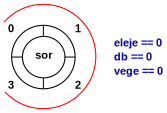
\includegraphics[width=\textwidth]{sor/sor01.pdf}
  \end{columns}
\end{frame}

%36
\begin{frame}
  \begin{columns}[c]
    \column{0.4\textwidth}
      \scriptsize
      \begin{exampleblock}{\textattachfile{sor2.cpp}{sor2.cpp}}
        \meret{7}
        \vspace{-.2cm}
        \lstinputlisting[style=cpp,linerange={4-24},numbers=left,firstnumber=4]{sor2.cpp}
        \vspace{-.2cm}
      \end{exampleblock}
    \column{0.55\textwidth}
      \includegraphics[width=\textwidth]{sor/sor02.pdf}
  \end{columns}
\end{frame}

%37
\begin{frame}
  \begin{columns}[c]
    \column{0.4\textwidth}
      \scriptsize
      \begin{exampleblock}{\textattachfile{sor2.cpp}{sor2.cpp}}
        \meret{7}
        \vspace{-.2cm}
        \lstinputlisting[style=cpp,linerange={4-24},numbers=left,firstnumber=4]{sor2.cpp}
        \vspace{-.2cm}
      \end{exampleblock}
    \column{0.55\textwidth}
      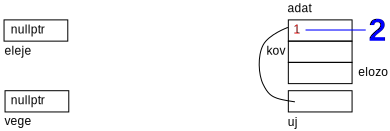
\includegraphics[width=\textwidth]{sor/sor03.pdf}
  \end{columns}
\end{frame}

%38
\begin{frame}
  \begin{columns}[c]
    \column{0.4\textwidth}
      \scriptsize
      \begin{exampleblock}{\textattachfile{sor2.cpp}{sor2.cpp}}
        \meret{7}
        \vspace{-.2cm}
        \lstinputlisting[style=cpp,linerange={4-24},numbers=left,firstnumber=4]{sor2.cpp}
        \vspace{-.2cm}
      \end{exampleblock}
    \column{0.55\textwidth}
      \includegraphics[width=\textwidth]{sor/sor04.pdf}
  \end{columns}
\end{frame}

%39
\begin{frame}
  \begin{columns}[c]
    \column{0.4\textwidth}
      \scriptsize
      \begin{exampleblock}{\textattachfile{sor2.cpp}{sor2.cpp}}
        \meret{7}
        \vspace{-.2cm}
        \lstinputlisting[style=cpp,linerange={4-24},numbers=left,firstnumber=4]{sor2.cpp}
        \vspace{-.2cm}
      \end{exampleblock}
    \column{0.55\textwidth}
      \includegraphics[width=\textwidth]{sor/sor05.pdf}
  \end{columns}
\end{frame}

%40
\begin{frame}
  \begin{columns}[c]
    \column{0.4\textwidth}
      \scriptsize
      \begin{exampleblock}{\textattachfile{sor2.cpp}{sor2.cpp}}
        \meret{7}
        \vspace{-.2cm}
        \lstinputlisting[style=cpp,linerange={4-24},numbers=left,firstnumber=4]{sor2.cpp}
        \vspace{-.2cm}
      \end{exampleblock}
    \column{0.55\textwidth}
      \includegraphics[width=\textwidth]{sor/sor06.pdf}
  \end{columns}
\end{frame}

%41
\begin{frame}
  \begin{columns}[c]
    \column{0.4\textwidth}
      \scriptsize
      \begin{exampleblock}{\textattachfile{sor2.cpp}{sor2.cpp}}
        \meret{7}
        \vspace{-.2cm}
        \lstinputlisting[style=cpp,linerange={4-24},numbers=left,firstnumber=4]{sor2.cpp}
        \vspace{-.2cm}
      \end{exampleblock}
    \column{0.55\textwidth}
      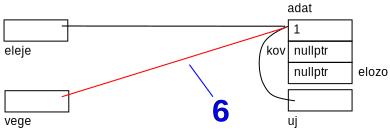
\includegraphics[width=\textwidth]{sor/sor07.pdf}
  \end{columns}
\end{frame}

%42
\begin{frame}
  \begin{columns}[c]
    \column{0.4\textwidth}
      \scriptsize
      \begin{exampleblock}{\textattachfile{sor2.cpp}{sor2.cpp}}
        \meret{7}
        \vspace{-.2cm}
        \lstinputlisting[style=cpp,linerange={4-24},numbers=left,firstnumber=4]{sor2.cpp}
        \vspace{-.2cm}
      \end{exampleblock}
    \column{0.55\textwidth}
      \includegraphics[width=\textwidth]{sor/sor08.pdf}
  \end{columns}
\end{frame}

%43
\begin{frame}
  \begin{columns}[c]
    \column{0.4\textwidth}
      \scriptsize
      \begin{exampleblock}{\textattachfile{sor2.cpp}{sor2.cpp}}
        \meret{7}
        \vspace{-.2cm}
        \lstinputlisting[style=cpp,linerange={4-24},numbers=left,firstnumber=4]{sor2.cpp}
        \vspace{-.2cm}
      \end{exampleblock}
    \column{0.55\textwidth}
      \includegraphics[width=\textwidth]{sor/sor09.pdf}
  \end{columns}
\end{frame}

%44
\begin{frame}
  \begin{columns}[c]
    \column{0.4\textwidth}
      \scriptsize
      \begin{exampleblock}{\textattachfile{sor2.cpp}{sor2.cpp}}
        \meret{7}
        \vspace{-.2cm}
        \lstinputlisting[style=cpp,linerange={4-24},numbers=left,firstnumber=4]{sor2.cpp}
        \vspace{-.2cm}
      \end{exampleblock}
    \column{0.55\textwidth}
      
\includegraphics[width=\textwidth]{sor/sor10.pdf}
  \end{columns}
\end{frame}

%45
\begin{frame}
  \begin{columns}[c]
    \column{0.4\textwidth}
      \scriptsize
      \begin{exampleblock}{\textattachfile{sor2.cpp}{sor2.cpp}}
        \meret{7}
        \vspace{-.2cm}
        \lstinputlisting[style=cpp,linerange={4-24},numbers=left,firstnumber=4]{sor2.cpp}
        \vspace{-.2cm}
      \end{exampleblock}
    \column{0.55\textwidth}
      \includegraphics[width=\textwidth]{sor/sor11.pdf}
  \end{columns}
\end{frame}

%46
\begin{frame}
  \begin{columns}[c]
    \column{0.4\textwidth}
      \scriptsize
      \begin{exampleblock}{\textattachfile{sor2.cpp}{sor2.cpp}}
        \meret{7}
        \vspace{-.2cm}
        \lstinputlisting[style=cpp,linerange={4-24},numbers=left,firstnumber=4]{sor2.cpp}
        \vspace{-.2cm}
      \end{exampleblock}
    \column{0.55\textwidth}
      \includegraphics[width=\textwidth]{sor/sor12.pdf}
  \end{columns}
\end{frame}

%47
\begin{frame}
  \begin{columns}[c]
    \column{0.4\textwidth}
      \scriptsize
      \begin{exampleblock}{\textattachfile{sor2.cpp}{sor2.cpp}}
        \meret{7}
        \vspace{-.2cm}
        \lstinputlisting[style=cpp,linerange={4-24},numbers=left,firstnumber=4]{sor2.cpp}
        \vspace{-.2cm}
      \end{exampleblock}
    \column{0.55\textwidth}
      \includegraphics[width=\textwidth]{sor/sor13.pdf}
  \end{columns}
\end{frame}

%48
\begin{frame}
  \begin{columns}[c]
    \column{0.4\textwidth}
      \scriptsize
      \begin{exampleblock}{\textattachfile{sor2.cpp}{sor2.cpp}}
        \meret{7}
        \vspace{-.2cm}
        \lstinputlisting[style=cpp,linerange={4-24},numbers=left,firstnumber=4]{sor2.cpp}
        \vspace{-.2cm}
      \end{exampleblock}
    \column{0.55\textwidth}
      \includegraphics[width=\textwidth]{sor/sor14.pdf}
  \end{columns}
\end{frame}

%%%%%%%%%%%%%%%%%%%%%%%%%%%%%%%%%%%
%%%%%%%%%%%%%%%%%%%%%%%%%%%%%%%%%%%

%49
\subsection{Elemek eltávolítása a sorból (dequeue)}
\begin{frame}
  \begin{columns}[c]
    \column{0.52\textwidth}
      \scriptsize
      \begin{exampleblock}{\textattachfile{sor2.cpp}{sor2.cpp}}
        \scriptsize
        \lstinputlisting[style=cpp,linerange={26-41},numbers=left,firstnumber=26]{sor2.cpp}
      \end{exampleblock}
    \column{0.43\textwidth}
      \includegraphics[width=\textwidth]{sor/sor20.pdf}
  \end{columns}
\end{frame}

%50
\begin{frame}
  \begin{columns}[c]
    \column{0.52\textwidth}
      \scriptsize
      \begin{exampleblock}{\textattachfile{sor2.cpp}{sor2.cpp}}
        \scriptsize
        \lstinputlisting[style=cpp,linerange={26-41},numbers=left,firstnumber=26]{sor2.cpp}
      \end{exampleblock}
    \column{0.43\textwidth}
      \includegraphics[width=\textwidth]{sor/sor21.pdf}
  \end{columns}
\end{frame}

%51
\begin{frame}
  \begin{columns}[c]
    \column{0.52\textwidth}
      \scriptsize
      \begin{exampleblock}{\textattachfile{sor2.cpp}{sor2.cpp}}
        \scriptsize
        \lstinputlisting[style=cpp,linerange={26-41},numbers=left,firstnumber=26]{sor2.cpp}
      \end{exampleblock}
    \column{0.43\textwidth}
      \includegraphics[width=\textwidth]{sor/sor22.pdf}
  \end{columns}
\end{frame}

%52
\begin{frame}
  \begin{columns}[c]
    \column{0.52\textwidth}
      \scriptsize
      \begin{exampleblock}{\textattachfile{sor2.cpp}{sor2.cpp}}
        \scriptsize
        \lstinputlisting[style=cpp,linerange={26-41},numbers=left,firstnumber=26]{sor2.cpp}
      \end{exampleblock}
    \column{0.43\textwidth}
      \includegraphics[width=\textwidth]{sor/sor23.pdf}
  \end{columns}
\end{frame}

%53
\begin{frame}
  \begin{columns}[c]
    \column{0.52\textwidth}
      \scriptsize
      \begin{exampleblock}{\textattachfile{sor2.cpp}{sor2.cpp}}
        \scriptsize
        \lstinputlisting[style=cpp,linerange={26-41},numbers=left,firstnumber=26]{sor2.cpp}
      \end{exampleblock}
    \column{0.43\textwidth}
      \includegraphics[width=\textwidth]{sor/sor24.pdf}
  \end{columns}
\end{frame}

%54
\begin{frame}
  \begin{columns}[c]
    \column{0.52\textwidth}
      \scriptsize
      \begin{exampleblock}{\textattachfile{sor2.cpp}{sor2.cpp}}
        \scriptsize
        \lstinputlisting[style=cpp,linerange={26-41},numbers=left,firstnumber=26]{sor2.cpp}
      \end{exampleblock}
    \column{0.43\textwidth}
      \includegraphics[width=\textwidth]{sor/sor25.pdf}
  \end{columns}
\end{frame}

%55
\begin{frame}
  \begin{columns}[c]
    \column{0.52\textwidth}
      \scriptsize
      \begin{exampleblock}{\textattachfile{sor2.cpp}{sor2.cpp}}
        \scriptsize
        \lstinputlisting[style=cpp,linerange={26-41},numbers=left,firstnumber=26]{sor2.cpp}
      \end{exampleblock}
    \column{0.43\textwidth}
      \includegraphics[width=\textwidth]{sor/sor26.pdf}
  \end{columns}
\end{frame}

%56
\begin{frame}
  \begin{columns}[c]
    \column{0.52\textwidth}
      \scriptsize
      \begin{exampleblock}{\textattachfile{sor2.cpp}{sor2.cpp}}
        \scriptsize
        \lstinputlisting[style=cpp,linerange={26-41},numbers=left,firstnumber=26]{sor2.cpp}
      \end{exampleblock}
    \column{0.43\textwidth}
      \includegraphics[width=\textwidth]{sor/sor27.pdf}
  \end{columns}
\end{frame}

%57
\begin{frame}
  \begin{columns}[c]
    \column{0.52\textwidth}
      \scriptsize
      \begin{exampleblock}{\textattachfile{sor2.cpp}{sor2.cpp}}
        \scriptsize
        \lstinputlisting[style=cpp,linerange={26-41},numbers=left,firstnumber=26]{sor2.cpp}
      \end{exampleblock}
    \column{0.43\textwidth}
      \includegraphics[width=\textwidth]{sor/sor28.pdf}
  \end{columns}
\end{frame}

%58
\begin{frame}
  \begin{columns}[c]
    \column{0.52\textwidth}
      \scriptsize
      \begin{exampleblock}{\textattachfile{sor2.cpp}{sor2.cpp}}
        \scriptsize
        \lstinputlisting[style=cpp,linerange={26-41},numbers=left,firstnumber=26]{sor2.cpp}
      \end{exampleblock}
    \column{0.43\textwidth}
      \includegraphics[width=\textwidth]{sor/sor29.pdf}
  \end{columns}
\end{frame}

%%%%%%%%%%%%%%%%%%%%%%%%%%%%%%%%%%%
%%%%%%%%%%%%%%%%%%%%%%%%%%%%%%%%%%%

%59
\subsection{Néhány általános listaművelet megvalósítása}
\begin{frame}
  Készítsünk ismét általános célú függvényeket!
  \begin{exampleblock}{\textattachfile{listaTeszt2.cpp}{listaTeszt2.cpp} %
(\textattachfile{Lista2.cpp}{Lista2.cpp}, \textattachfile{Lista2.h}{Lista2.h})}
    \footnotesize
    \vspace{-.2cm}
    \lstinputlisting[style=cpp,linerange={5-17},numbers=left,firstnumber=5]{listaTeszt2.cpp}
    \vspace{-.2cm}
  \end{exampleblock}
\end{frame}

%%%%%%%%%%%%%%%%%%%%%%%%%%%%%%%%%%%
%%%%%%%%%%%%%%%%%%%%%%%%%%%%%%%%%%%

%60
\subsection{Új elem beillesztése adott elem után}
\begin{frame}
  \begin{columns}[c]
    \column{0.5\textwidth}
      \scriptsize
      \begin{exampleblock}{\textattachfile{Lista2.cpp}{Lista2.cpp}}
        \vspace{-.2cm}
        \lstinputlisting[style=cpp,linerange={4-20},numbers=left,firstnumber=4]{Lista2.cpp}
        \vspace{-.2cm}
    \end{exampleblock}
    \column{0.45\textwidth}
      \includegraphics[width=\textwidth]{lista2/list2-1.pdf}
  \end{columns}
\end{frame}

%61
\begin{frame}
  \begin{columns}[c]
    \column{0.5\textwidth}
      \scriptsize
      \begin{exampleblock}{\textattachfile{Lista2.cpp}{Lista2.cpp}}
        \vspace{-.2cm}
        \lstinputlisting[style=cpp,linerange={4-20},numbers=left,firstnumber=4]{Lista2.cpp}
        \vspace{-.2cm}
    \end{exampleblock}
    \column{0.45\textwidth}
      \includegraphics[width=\textwidth]{lista2/list2-2.pdf}
  \end{columns}
\end{frame}

%62
\begin{frame}
  \begin{columns}[c]
    \column{0.5\textwidth}
      \scriptsize
      \begin{exampleblock}{\textattachfile{Lista2.cpp}{Lista2.cpp}}
        \vspace{-.2cm}
        \lstinputlisting[style=cpp,linerange={4-20},numbers=left,firstnumber=4]{Lista2.cpp}
        \vspace{-.2cm}
    \end{exampleblock}
    \column{0.45\textwidth}
      \includegraphics[width=\textwidth]{lista2/list2-3.pdf}
  \end{columns}
\end{frame}

%63
\begin{frame}
  \begin{columns}[c]
    \column{0.5\textwidth}
      \scriptsize
      \begin{exampleblock}{\textattachfile{Lista2.cpp}{Lista2.cpp}}
        \vspace{-.2cm}
        \lstinputlisting[style=cpp,linerange={4-20},numbers=left,firstnumber=4]{Lista2.cpp}
        \vspace{-.2cm}
    \end{exampleblock}
    \column{0.45\textwidth}
      \includegraphics[width=\textwidth]{lista2/list2-4.pdf}
  \end{columns}
\end{frame}

%64
\begin{frame}
  \begin{columns}[c]
    \column{0.5\textwidth}
      \scriptsize
      \begin{exampleblock}{\textattachfile{Lista2.cpp}{Lista2.cpp}}
        \vspace{-.2cm}
        \lstinputlisting[style=cpp,linerange={4-20},numbers=left,firstnumber=4]{Lista2.cpp}
        \vspace{-.2cm}
    \end{exampleblock}
    \column{0.45\textwidth}
      \includegraphics[width=\textwidth]{lista2/list2-5.pdf}
  \end{columns}
\end{frame}

%65
\begin{frame}
  \begin{columns}[c]
    \column{0.5\textwidth}
      \scriptsize
      \begin{exampleblock}{\textattachfile{Lista2.cpp}{Lista2.cpp}}
        \vspace{-.2cm}
        \lstinputlisting[style=cpp,linerange={4-20},numbers=left,firstnumber=4]{Lista2.cpp}
        \vspace{-.2cm}
    \end{exampleblock}
    \column{0.45\textwidth}
      \includegraphics[width=\textwidth]{lista2/list2-6.pdf}
  \end{columns}
\end{frame}

%%%%%%%%%%%%%%%%%%%%%%%%%%%%%%%%%%%
%%%%%%%%%%%%%%%%%%%%%%%%%%%%%%%%%%%

%66
\begin{frame}[fragile]
  \begin{exampleblock}{\textattachfile{listaTeszt2.cpp}{listaTeszt2.cpp} %
(\textattachfile{Lista2.cpp}{Lista2.cpp}, \textattachfile{Lista2.h}{Lista2.h})}
    \small
    \vspace{-.2cm}
    \lstinputlisting[style=cpp,linerange={18-24},numbers=left,firstnumber=18]{listaTeszt2.cpp}
    \vspace{-.2cm}
  \end{exampleblock}
  \begin{block}{Kimenet}
    \small
    \vspace{-.2cm}
    \begin{verbatim}
0       1       2       3       4       5       6       
0       1       2       3       666     4       5       6       
1       2       3       4       5       6
\end{verbatim}
    \vspace{-.2cm}
  \end{block}
\end{frame}

%%%%%%%%%%%%%%%%%%%%%%%%%%%%%%%%%%%
%%%%%%%%%%%%%%%%%%%%%%%%%%%%%%%%%%%

%67
\subsection{Elem törlése kétszeresen láncolt listából}
\begin{frame}
  \begin{center}
    \includegraphics[scale=0.55]{lista2/list2-10.pdf}
  \end{center}
  \vspace{-.4cm}
  \scriptsize
  \begin{exampleblock}{\textattachfile{Lista2.cpp}{Lista2.cpp}}
    \tiny
    \vspace{-.2cm}
    \lstinputlisting[style=cpp,linerange={30-40},numbers=left,firstnumber=30]{Lista2.cpp}
    \vspace{-.2cm}
  \end{exampleblock}
\end{frame}

%68
\begin{frame}
  \begin{center}
    \includegraphics[scale=0.55]{lista2/list2-11.pdf}
  \end{center}
  \vspace{-.4cm}
  \scriptsize
  \begin{exampleblock}{\textattachfile{Lista2.cpp}{Lista2.cpp}}
    \tiny
    \vspace{-.2cm}
    \lstinputlisting[style=cpp,linerange={30-40},numbers=left,firstnumber=30]{Lista2.cpp}
    \vspace{-.2cm}
  \end{exampleblock}
\end{frame}

%69
\begin{frame}
  \begin{center}
    \includegraphics[scale=0.55]{lista2/list2-12.pdf}
  \end{center}
  \vspace{-.4cm}
  \scriptsize
  \begin{exampleblock}{\textattachfile{Lista2.cpp}{Lista2.cpp}}
    \tiny
    \vspace{-.2cm}
    \lstinputlisting[style=cpp,linerange={30-40},numbers=left,firstnumber=30]{Lista2.cpp}
    \vspace{-.2cm}
  \end{exampleblock}
\end{frame}

%70
\begin{frame}
  \begin{center}
    \includegraphics[scale=0.55]{lista2/list2-13.pdf}
  \end{center}
  \vspace{-.4cm}
  \scriptsize
  \begin{exampleblock}{\textattachfile{Lista2.cpp}{Lista2.cpp}}
    \tiny
    \vspace{-.2cm}
    \lstinputlisting[style=cpp,linerange={30-40},numbers=left,firstnumber=30]{Lista2.cpp}
    \vspace{-.2cm}
  \end{exampleblock}
\end{frame}

%71
\begin{frame}
  \begin{center}
    \includegraphics[scale=0.55]{lista2/list2-14.pdf}
  \end{center}
  \vspace{-.4cm}
  \scriptsize
  \begin{exampleblock}{\textattachfile{Lista2.cpp}{Lista2.cpp}}
    \tiny
    \vspace{-.2cm}
    \lstinputlisting[style=cpp,linerange={30-40},numbers=left,firstnumber=30]{Lista2.cpp}
    \vspace{-.2cm}
  \end{exampleblock}
\end{frame}

%72
\begin{frame}
  \begin{center}
    \includegraphics[scale=0.55]{lista2/list2-15.pdf}
  \end{center}
  \vspace{-.4cm}
  \scriptsize
  \begin{exampleblock}{\textattachfile{Lista2.cpp}{Lista2.cpp}}
    \tiny
    \vspace{-.2cm}
    \lstinputlisting[style=cpp,linerange={30-40},numbers=left,firstnumber=30]{Lista2.cpp}
    \vspace{-.2cm}
  \end{exampleblock}
\end{frame}

%%%%%%%%%%%%%%%%%%%%%%%%%%%%%%%%%%%
%%%%%%%%%%%%%%%%%%%%%%%%%%%%%%%%%%%

%73
\subsection{Kétszeresen láncolt lista bejárása, törlése}
\begin{frame}
  \begin{exampleblock}{\textattachfile{Lista2.cpp}{Lista2.cpp}}
    \footnotesize
    \vspace{-.2cm}
    \lstinputlisting[style=cpp,linerange={42-48},numbers=left,firstnumber=42]{Lista2.cpp}
    \lstinputlisting[style=cpp,linerange={22-28},numbers=left,firstnumber=22]{Lista2.cpp}
    \vspace{-.2cm}
  \end{exampleblock}
\end{frame}

\end{document}